\chapter{Binäärihakupuu}

Binäärihakupuu on tietorakenne, joka pitää yllä alkioiden joukkoa.
Binääri\-hakupuun perusoperaatiot ovat samat kuin hajautustaulussa:

\begin{itemize}
\item lisää alkio $x$ joukkoon
\item tarkista, onko alkio $x$ joukossa
\item poista alkio $x$ joukosta
\end{itemize}

Koska binäärihakupuu säilyttää joukon alkioita
\emph{järjestyksessä}, voimme toteuttaa lisäksi tehokkaasti
esimerkiksi seuraavat operaatiot:

\begin{itemize}
\item etsi joukon pienin/suurin alkio
\item etsi joukon pienin alkio, joka on vähintään $x$
\item etsi joukon suurin alkio, joka on enintään $x$
\end{itemize}

Hajautustaulu \emph{ei} pysty tarjoamaan tällaisia operaatioita
tehokkaasti, joten binäärihakupuu on hyvä valinta, jos näille
operaatioille on tarvetta joukon perusoperaatioiden lisäksi.

Voimme toteuttaa binäärihakupuun niin,
että kaikki sen operaatiot toimivat ajassa $O(\log n)$.
Tämä vaatii, että puu on \emph{tasapainoinen},
minkä saavuttamiseksi on monia menetelmiä.
Tässä luvussa tutustumme AVL-puuhun, joka on
yksinkertainen esimerkki tasapainoisesta binääripuusta.
Javan tietorakenteet perustuvat taas punamustaan puuhun,
joka on AVL-puuta vaikeampi toteuttaa mutta tietyissä tilanteissa tehokkaampi.

\section{Taustaa binääripuista}

Binäärihakupuun taustalla on yleisempi tietorakenne \emph{binääripuu}.
Ennen kuin tutustumme binäärihakupuuhun,
meidän onkin hyvä tietää ensin, mikä on binääripuu ja mitä
ominaisuuksia siihen liittyy.

Binääripuu muodostuu $n$ solmusta, jotka on yhdistetty toisiinsa.
Puussa ylimpänä on solmu, jota kutsutaan \emph{juureksi}.
Jokaisella solmulla voi olla vasen ja oikea \emph{lapsi},
ja kaikilla solmuilla juurta lukuun ottamatta on yksikäsitteinen \emph{vanhempi}.
Puun \emph{lehtiä} ovat solmut, joilla ei ole lapsia.

Binääripuun rakenne on rekursiivinen:
jokainen solmu toimii juurena \emph{alipuulle},
joka on myös binääripuu.
Voimmekin myös ajatella, että binääripuun
solmun vasen ja oikea lapsi on joko tyhjä
tai toinen binääripuu.

\begin{figure}
\center
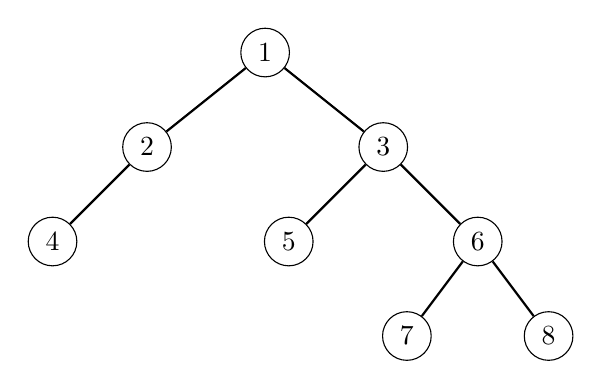
\begin{tikzpicture}[scale=0.6]
\node[draw, circle] (1) at (0,0) {$1$};
\node[draw, circle] (2) at (-2.5,-2) {$2$};
\node[draw, circle] (3) at (2.5,-2) {$3$};
\node[draw, circle] (4) at (-4.5,-4) {$4$};
\node[draw, circle] (5) at (0.5,-4) {$5$};
\node[draw, circle] (6) at (4.5,-4) {$6$};
\node[draw, circle] (7) at (3,-6) {$7$};
\node[draw, circle] (8) at (6,-6) {$8$};
\path[draw,thick,-] (1) -- (2);
\path[draw,thick,-] (1) -- (3);
\path[draw,thick,-] (2) -- (4);
\path[draw,thick,-] (3) -- (5);
\path[draw,thick,-] (3) -- (6);
\path[draw,thick,-] (6) -- (7);
\path[draw,thick,-] (6) -- (8);
\end{tikzpicture}
\caption{Binääripuu, jossa on 8 solmua.}
\label{fig:binpuu}
\end{figure}

Kuvassa \ref{fig:binpuu} on esimerkki binääripuusta, jossa on 8 solmua.
Solmu 1 on puun juuri, ja solmut 4, 5, 7 ja 8 ovat puun lehtiä.
Solmun 3 vasen lapsi on solmu 5, oikea lapsi on solmu 6
ja vanhempi on solmu 1.
Solmun 3 alipuussa ovat solmut 3, 5, 6, 7 ja 8.

Binääripuun juuren \emph{syvyys} on 0 ja jokaisen muun solmun syvyys on yhtä
suurempi kuin sen vanhemman syvyys.
Binääripuun \emph{korkeus} on puolestaan suurin puun solmussa
esiintyvä syvyys.
Esimerkiksi kuvan \ref{fig:binpuu} puun korkeus on 3,
koska solmujen 7 ja 8 syvyys on 3.

\subsection{Binääripuun käsittely}

Voimme toteuttaa binääripuun linkitettynä rakenteena niin,
että jokainen puun solmu on olio, josta on viittaus
solmun vasempaan ja oikeaan lapseen.
Javassa voimme määritellä solmua vastaavan luokan seuraavasti:

\begin{code}
public class Node {
    Node left, right;
    int value;

    public Node(Node left, Node right, int value) {
        this.left = left;
        this.right = right;
        this.value = value;
    }
}
\end{code}

Kentät \texttt{left} ja \texttt{right} osoittavat solmun
vasempaan ja oikeaan lapseen.
Jos lapsi puuttuu, sen tilalla on arvo \texttt{null}.
Kentässä \texttt{value} on puolestaan solmun arvo.
Nyt voimme määritellä kuvan \ref{fig:binpuu} binääripuun näin:

\begin{code}
Node node4 = new Node(null, null, 4);
Node node2 = new Node(node4, null, 2);
Node node7 = new Node(null, null, 7);
Node node8 = new Node(null, null, 8);
Node node6 = new Node(node7, node8, 6);
Node node5 = new Node(null, null, 5);
Node node3 = new Node(node5, node6, 3);
Node node1 = new Node(node2, node3, 1);
\end{code}

Voimme toteuttaa monia binääripuun käsittelyyn liittyviä
operaatioita luontevasti rekursiolla.
Esimerkiksi seuraava metodi laskee, montako solmua
sille annetussa puussa on:

\begin{code}
int laskeSolmut(Node puu) {
    if (puu == null) return 0;
    return 1 + laskeSolmut(puu.left) + laskeSolmut(puu.right);
}
\end{code}

Seuraava metodi puolestaan selvittää, mikä on puun korkeus:

\begin{code}
int korkeus(Node puu) {
    if (puu == null) return -1;
    return 1 + Math.max(korkeus(puu.left), korkeus(puu.right));
}
\end{code}

Huomaa, että jos puu on tyhjä, meidän on kätevää tulkita,
että sen korkeus on $-1$.

\subsection{Läpikäyntijärjestykset}

Voimme käydä läpi binääripuun solmut rekursiivisesti
juuresta alkaen.
Solmujen läpikäyntiin on kolme tavallista järjestystä:

\begin{itemize}
\item \emph{esijärjestys}: käsittelemme ensin solmun, sitten vasemman alipuun
ja lopuksi oikean alipuun
\item \emph{sisäjärjestys}: käsittelemme ensin vasemman alipuun, sitten solmun
ja lopuksi oikean alipuun
\item \emph{jälkijärjestys}: käsittelemme ensin vasemman alipuun,
sitten oikean alipuun ja lopuksi solmun
\end{itemize}

Esimerkiksi kuvan \ref{fig:binpuu} puussa
esijärjestys on $[1,2,4,3,5,6,7,8]$,
sisäjärjes\-tys on $[4,2,1,5,3,7,6,8]$ ja
jälkijärjestys on $[4,2,5,7,8,6,3,1]$.

Seuraava metodi tulostaa binääripuun solmut
sisäjärjestyksessä, kun sille annetaan parametrina
puun juuri.

\begin{code}
void traverse(Node puu) {
    if (puu == null) return;
    traverse(puu.left);
    System.out.println(puu.value);
    traverse(puu.right);
}
\end{code}

\section{Binäärihakupuun toteutus}

Binäärihakupuu on binääripuu, jonka jokainen solmu
on yksi joukon alkioista.
Solmut on järjestetty niin, että jokaisessa solmussa
kaikki arvot vasemmassa alipuussa ovat pienempiä
kuin solmun arvo ja vastaavasti kaikki arvot 
oikeassa alipuussa ovat suurempia.
Tämän ominaisuuden ansiosta voimme löytää helposti
alkion puusta aloittamalla haun puun juuresta.

\begin{figure}
\center
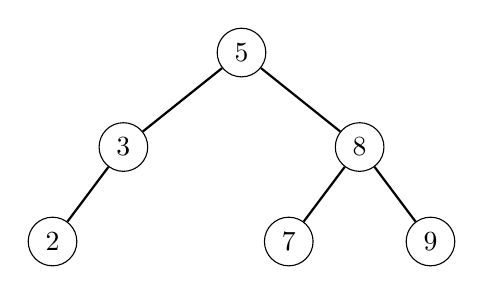
\begin{tikzpicture}[scale=0.6]
\node[draw, circle] (1) at (0,0) {$5$};
\node[draw, circle] (2) at (-2.5,-2) {$3$};
\node[draw, circle] (3) at (2.5,-2) {$8$};
\node[draw, circle] (4) at (-4,-4) {$2$};
\node[draw, circle] (5) at (1,-4) {$7$};
\node[draw, circle] (6) at (4,-4) {$9$};
\path[draw,thick,-] (1) -- (2);
\path[draw,thick,-] (1) -- (3);
\path[draw,thick,-] (2) -- (4);
\path[draw,thick,-] (3) -- (5);
\path[draw,thick,-] (3) -- (6);
\end{tikzpicture}
\caption{Joukkoa $\{2,3,5,7,8,9\}$ vastaava binäärihakupuu.}
\label{fig:bihpuu}
\end{figure}

Kuvassa \ref{fig:bihpuu} on binäärihakupuu,
joka vastaa joukkoa $\{2,3,5,7,8,9\}$.
Tässä tapauksessa puun juuren arvo on 5,
joten vasemmassa alipuussa kaikki arvot
ovat pienempiä kuin 5 ja oikeassa alipuussa
kaikki arvot ovat suurempia kuin 5.
Sama ehto pätee kaikissa muissakin puun solmuissa.

Seuraavaksi käymme läpi, kuinka voimme toteuttaa
haluamamme joukko-operaatiot
binäärihakupuun avulla.
Jokainen operaatio vie aikaa $O(h)$,
missä $h$ on puun korkeus.

\subsection{Joukko-operaatiot}

\subsubsection{Alkion etsiminen}

Kun haluamme löytää puusta solmun $x$, lähdemme liikkeelle
puun juuresta ja kuljemme rekursiivisesti alaspäin puussa.
Kun olemme solmussa, jonka arvo on $a$,
vaihtoehtoja on kolme.
Jos $a=x$, olemme löytäneet halutun solmun,
jos $a<x$, jatkamme hakua solmun oikeaan lapseen,
ja jos $a>x$, jatkamme hakua solmun vasempaan lapseen.
Kuitenkin jos haluttua lasta ei ole, toteamme,
että solmua $x$ ei esiinny puussa.

\begin{figure}
\center
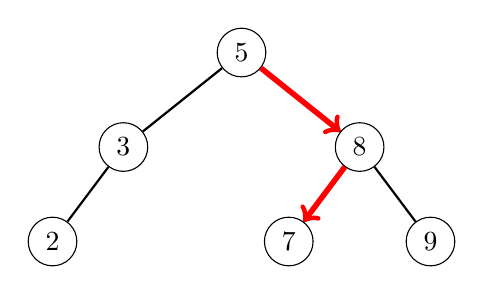
\begin{tikzpicture}[scale=0.6]
\node[draw, circle] (1) at (0,0) {$5$};
\node[draw, circle] (2) at (-2.5,-2) {$3$};
\node[draw, circle] (3) at (2.5,-2) {$8$};
\node[draw, circle] (4) at (-4,-4) {$2$};
\node[draw, circle] (5) at (1,-4) {$7$};
\node[draw, circle] (6) at (4,-4) {$9$};
\path[draw,thick,-] (1) -- (2);
\path[draw,thick,-] (1) -- (3);
\path[draw,thick,-] (2) -- (4);
\path[draw,thick,-] (3) -- (5);
\path[draw,thick,-] (3) -- (6);
\path[draw,thick,red,line width=2pt,->] (1) -- (3);
\path[draw,thick,red,line width=2pt,->] (3) -- (5);
\end{tikzpicture}
\caption{Alkion $7$ etsiminen joukosta $\{2,3,5,7,8,9\}$ juuresta alkaen.}
\label{fig:bihets}
\end{figure}

Kuva \ref{fig:bihets} näyttää, kuinka löydämme alkion 7
joukosta $\{2,3,5,7,8,9\}$.
Juuren arvona on 5, joten alkion täytyy olla juuren
oikeassa alipuussa.
Tämän solmun arvona on 8,
joten nyt taas tiedämme, että alkion täytyy olla
vasemmassa alipuussa, josta se löytyykin.

\subsubsection{Alkion lisääminen}

Kun haluamme lisätä puuhun solmun $x$, kuljemme ensin
puussa aivan kuin etsisimme solmua $x$.
Sitten kun olemme päässeet solmuun,
jolla ei ole lasta, johon meidän tulisi edetä,
lisäämme solmun $x$ tällaiseksi lapseksi.

\begin{figure}
\center
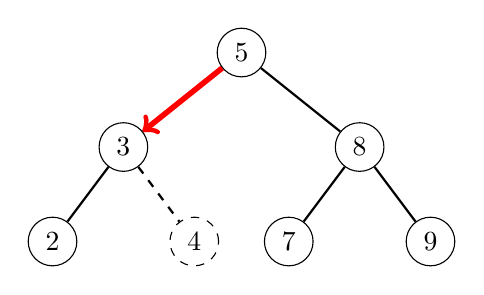
\begin{tikzpicture}[scale=0.6]
\node[draw, circle] (1) at (0,0) {$5$};
\node[draw, circle] (2) at (-2.5,-2) {$3$};
\node[draw, circle] (3) at (2.5,-2) {$8$};
\node[draw, circle] (4) at (-4,-4) {$2$};
\node[draw, circle] (5) at (1,-4) {$7$};
\node[draw, circle] (6) at (4,-4) {$9$};
\node[draw, circle, dashed] (7) at (-1,-4) {$4$};
\path[draw,thick,-] (1) -- (2);
\path[draw,thick,-] (1) -- (3);
\path[draw,thick,-] (2) -- (4);
\path[draw,thick,-] (3) -- (5);
\path[draw,thick,-] (3) -- (6);
\path[draw,thick,dashed,-] (2) -- (7);
\path[draw,thick,red,line width=2pt,->] (1) -- (2);
\end{tikzpicture}
\caption{Alkion 4 lisääminen joukkoon $\{2,3,5,7,8,9\}$.}
\label{fig:bihpu2}
\end{figure}

Kuva \ref{fig:bihpu2} näyttää, kuinka lisäämme alkion 4
joukkoon $\{2,3,5,7,8,9\}$.
Kun haemme puusta solmua 4, päädymme solmuun 3,
jolla ei ole oikeaa lasta.
Niinpä lisäämme solmun 4 solmun 3 oikeaksi lapseksi.

\subsubsection{Alkion poistaminen}

Kun haluamme poistaa puusta solmun $x$, etsimme ensin
solmun $x$ tavalliseen tapaan.
Jos solmulla $x$ ei ole lapsia, poistamme sen vain puusta.
Jos solmulla $x$ on yksi lapsi, korvaamme solmun $x$
sen lapsella.
Jos kuitenkin solmulla $x$ on kaksi lasta,
tilanne on hankalampi.
Tällöin etsimme puusta solmusta $x$ seuraavan
suuremman alkion $y$ (pian kuvattavalla tavalla), vaihdamme keskenään
solmujen $x$ ja $y$ arvot,
ja poistamme sitten solmun $y$.
Solmulla $y$ ei voi olla kahta lasta, joten poistaminen on helppoa.

\begin{figure}
\center
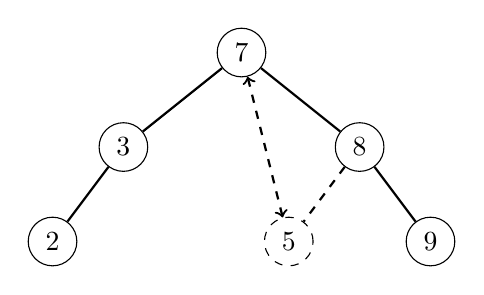
\begin{tikzpicture}[scale=0.6]
\node[draw, circle] (1) at (0,0) {$7$};
\node[draw, circle] (2) at (-2.5,-2) {$3$};
\node[draw, circle] (3) at (2.5,-2) {$8$};
\node[draw, circle] (4) at (-4,-4) {$2$};
\node[draw, circle, dashed] (5) at (1,-4) {$5$};
\node[draw, circle] (6) at (4,-4) {$9$};
\path[draw,thick,-] (1) -- (2);
\path[draw,thick,-] (1) -- (3);
\path[draw,thick,-] (2) -- (4);
\path[draw,thick,-,dashed] (3) -- (5);
\path[draw,thick,-] (3) -- (6);
\path[draw,thick,<->,dashed] (1) -- (5);
\end{tikzpicture}
\caption{Alkion 5 poistaminen joukosta $\{2,3,5,7,8,9\}$.}
\label{fig:bihpu3}
\end{figure}

Kuva \ref{fig:bihpu3} näyttää, kuinka poistamme joukosta $\{2,3,5,7,8,9\}$
alkion 5, joka vastaa binäärihakupuun juurta.
Solmun seuraava suurempi alkio on 7,
joten vaihdamme keskenään arvot 5 ja 7.
Tämän jälkeen meidän on helppoa poistaa solmu puusta.

\subsubsection{Pienin/suurin alkio}

Löydämme puun pienimmän alkion lähtemällä liikkeelle
puun juuresta ja siirtymällä vasempaan lapseen niin
kauan kuin tämä on mahdollista.
Solmu, johon päädymme lopulta, on puun pienin alkio.
Vastaavalla tavalla löydämme suurimman alkion
etenemällä koko ajan oikealle juuresta.

\subsubsection{Seuraava suurempi alkio}

Jos solmulla on oikea lapsi, siirrymme ensin solmusta oikealle
ja sitten vasemmalle niin kauan kuin mahdollista.
Muuten kuljemme solmusta ylöspäin, kunnes saavumme solmuun,
jonka vasen lapsi on edellinen lapsi.
Jos tällaista solmua ei ole, solmulla ei ole seuraavaa
suurempaa alkiota.

\subsubsection{Edellinen pienempi alkio}

Menettelemme käänteisesti edelliseen kohtaan nähden.

\subsection{Operaatioiden tehokkuus}

Binäärihakupuun operaatiot vievät aikaa $O(h)$,
missä $h$ on puun korkeus, joten operaatioiden tehokkuus
riippuu puun korkeudesta.
Niinpä puun tehokkuuteen vaikuttaa, miten olemme
rakentaneet sen.
Esimerkiksi kuvassa \ref{fig:bihkor} on kaksi mahdollista puuta
joukolle $\{1,2,3,4,5\}$.
Vasemman puun korkeus on 3, kun taas oikean puun korkeus on 5.

\begin{figure}
\center
\begin{tikzpicture}[scale=0.6]
\begin{scope}
\node[draw, circle] (1) at (0,0) {$1$};
\node[draw, circle] (2) at (1,-2) {$2$};
\node[draw, circle] (3) at (2,-4) {$3$};
\node[draw, circle] (4) at (3,-6) {$4$};
\node[draw, circle] (5) at (4,-8) {$5$};
\path[draw,thick,-] (1) -- (2);
\path[draw,thick,-] (2) -- (3);
\path[draw,thick,-] (3) -- (4);
\path[draw,thick,-] (4) -- (5);
\end{scope}
\begin{scope}[xshift=-8cm]
\node[draw, circle] (1) at (0,0) {$1$};
\node[draw, circle] (2) at (-2,-2) {$2$};
\node[draw, circle] (3) at (2,-2) {$3$};
\node[draw, circle] (4) at (-4,-4) {$4$};
\node[draw, circle] (5) at (0,-4) {$5$};
\path[draw,thick,-] (1) -- (2);
\path[draw,thick,-] (1) -- (3);
\path[draw,thick,-] (2) -- (4);
\path[draw,thick,-] (2) -- (5);
\end{scope}
\end{tikzpicture}
\caption{Kaksi binäärihakupuuta joukolle $\{1,2,3,4,5\}$.
Vasemman puun korkeus on 3, kun taas oikean puun korkeus on 5.}
\label{fig:bihkor}
\end{figure}


Jotta binäärihakupuu toimii tehokkaasti, haluamme,
että puun korkeus ei kasva liian suureksi.
Tarkemmin ottaen tavoitteemme on, että puun korkeus on
aina vain $O(\log n)$ eli puu on \emph{tasapainoinen}.
Jos onnistumme tässä, kaikki puun operaatiot toimivat
siis tehokkaasti ajassa $O(\log n)$.
Osoittautuu, että saavutamme tavoitteemme
lisäämällä puuhun ehtoja, jotka rajoittavat
sen korkeutta sopivasti.

Binäärihakupuun tasapainottamiseen tunnetaan monia menetelmiä.
Tutustumme seuraavaksi AVL-puuhun, joka on 
varhaisin tunnettu tasapainoinen binäärihakupuu.
AVL-puu on yksinkertaisempi kuin monet myöhemmin
kehitetyt rakenteet, minkä vuoksi se sopii hyvin esittelemään
puiden tasapainotuksen ideoita.
Javan ja muiden ohjelmointikielten standardikirjastoissa
käyte\-tään kuitenkin muita rakenteita, kuten punamustaa puuta.

\section{AVL-puu}

\emph{AVL-puu} on tasapainoinen binäärihakupuu, jonka
korkeus on aina $O(\log n)$, minkä ansiosta puun operaatiot
toimivat tehokkaasti ajassa $O(\log n)$.
AVL-puussa jokaiseen solmuun liittyy \emph{tasapainoehto},
joka takaa, että puu on tasapainoinen.
Kun päivitämme puuta, meidän täytyy pitää huolta siitä,
että tasapainoehto säilyy voimassa kaikissa solmuissa.

\subsection{Tasapainoehto}

AVL-puun tasapainoehto on, että
jokaisessa solmussa vasemman ja oikean lapsen alipuiden korkeusero 
on enintään 1.

Esimerkiksi kuvassa \ref{fig:bihkor} vasen puu on
AVL-puu, kun taas oikea puu ei ole.
Oikea puu ei ole AVL-puu, koska esimerkiksi solmussa 1
vasemman lapsen alipuun korkeus on 0 mutta oikean lapsen
alipuun korkeus on 4.
Korkeuksien erona on siis 4, vaikka ero saisi olla enintään 1.

Kutsumme AVL-puun tasapainoehtoa \emph{AVL-ehdoksi}.
Osoittautuu, että jos binäärihakupuu täyttää AVL-ehdon,
sen korkeus on $O(\log n)$.
Eli jos pystymme toteuttamaan puun operaatiot niin,
että AVL-ehto säilyy, saamme aikaan binäärihakupuun,
jonka operaatiot toimivat ajassa $O(\log n)$.

\begin{figure}
\center
\scriptsize
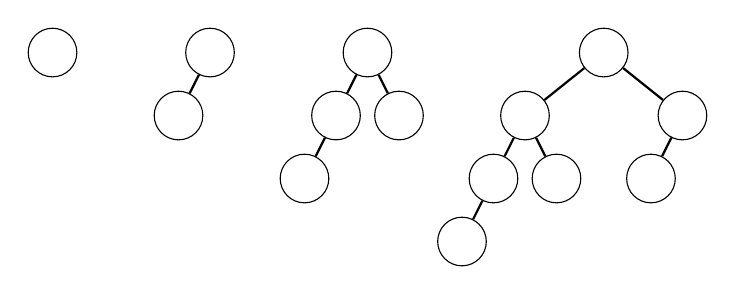
\begin{tikzpicture}[scale=0.4]
\begin{scope}
\node[draw, circle] (2) at (-2.5,-2) {\phantom{$1$}};
\end{scope}
\begin{scope}[xshift=5cm]
\node[draw, circle] (2) at (-2.5,-2) {\phantom{$1$}};
\node[draw, circle] (4) at (-3.5,-4) {\phantom{$1$}};
\path[draw,thick,-] (2) -- (4);
\end{scope}
\begin{scope}[xshift=10cm]
\node[draw, circle] (2) at (-2.5,-2) {\phantom{$1$}};
\node[draw, circle] (4) at (-3.5,-4) {\phantom{$1$}};
\node[draw, circle] (5) at (-1.5,-4) {\phantom{$1$}};
\node[draw, circle] (7) at (-4.5,-6) {\phantom{$1$}};
\path[draw,thick,-] (2) -- (4);
\path[draw,thick,-] (2) -- (5);
\path[draw,thick,-] (4) -- (7);
\end{scope}
\begin{scope}[xshift=15cm,yshift=-2cm]
\node[draw, circle] (1) at (0,0) {\phantom{$1$}};
\node[draw, circle] (2) at (-2.5,-2) {\phantom{$1$}};
\node[draw, circle] (3) at (2.5,-2) {\phantom{$1$}};
\node[draw, circle] (4) at (-3.5,-4) {\phantom{$1$}};
\node[draw, circle] (5) at (-1.5,-4) {\phantom{$1$}};
\node[draw, circle] (6) at (1.5,-4) {\phantom{$1$}};
\node[draw, circle] (7) at (-4.5,-6) {\phantom{$1$}};
\path[draw,thick,-] (1) -- (2);
\path[draw,thick,-] (1) -- (3);
\path[draw,thick,-] (2) -- (4);
\path[draw,thick,-] (2) -- (5);
\path[draw,thick,-] (3) -- (6);
\path[draw,thick,-] (4) -- (7);
\end{scope}
\end{tikzpicture}
\caption{Vähiten solmuja sisältävät AVL-puut korkeuksille 1, 2, 3 ja 4.}
\label{fig:avlkor}
\end{figure}

Miksi sitten AVL-ehto takaa, että binäärihakupuun korkeus
on $O(\log n)$?
Voimme lähestyä asiaa pahimman tapauksen kautta:
kun tiedämme, että AVL-puussa on $n$ solmua,
mikä on sen \emph{suurin mahdollinen} korkeus?
Voimme selvittää tämän tutkimalla käänteisesti,
mikä on \emph{pienin mahdollinen} solmujen määrä
AVL-puussa, jonka korkeus on $h$.

Merkitään $f(h)$:lla korkeutta $h$ olevan AVL-puun
pienintä mahdollista solmujen määrää.
Kuvan \ref{fig:avlkor} mukaisesti funktion ensimmäiset arvot
ovat $f(1)=1$, $f(2)=2$, $f(3)=4$ ja $f(4)=7$.
Yleisemmin
\[f(h)=f(h-1)+f(h-2)+1,\]
koska jos haluamme rakentaa AVL-puun korkeutta $h$,
jossa on mahdollisimman vähän solmuja,
meidän kannattaa laittaa juuren vasempaan
lapseen AVL-puu korkeutta $h-1$ ja oikeaan lapseen
AVL-puu korkeutta $h-2$ niin,
että kummassakin alipuussa on mahdollisimman vähän solmuja.

Kun $h \ge 3 $, funktiolle pätee
\[f(h) \ge 2 f(h-2),\]
eli funktion arvo ainakin kaksinkertaistuu kahden askeleen välein.
Voimme esittää tämän alarajan muodossa
\[f(h) \ge 2^{h/2},\]
joka taas tarkoittaa samaa kuin
\[ h \le 2 \log_2 f(h).\]

Tarkastellaan sitten puuta, jossa on $n$ solmua.
Puun korkeudelle $h$ täytyy päteä $f(h) \le n$,
koska korkeutta $h$ olevassa puussa on vähintään $f(h)$ solmua.
Niinpä saamme alarajan
\[h \le 2 \log_2 n,\]
mikä tarkoittaa samaa kuin $h = O(\log n)$.

\subsection{Kiertojen toteutus}

TODO

\section{Javan rakenteet}

Javan rakenteet \texttt{TreeSet} ja \texttt{TreeMap}
pohjautuvat binäärihakupuuhun.
Ne muistuttavat rakenteita \texttt{HashSet} ja \texttt{HashMap},
mutta erona on, että pystymme etsimään
alkioita niiden järjestyksen perusteella.

\subsection{\texttt{TreeSet}-rakenne}

Seuraava koodi luo \texttt{TreeSet}-rakenteen,
joka pitää yllä lukujen joukkoa.
Koodi lisää joukkoon alkioita ja tulostaa sitten sen sisällön.

\begin{code}
TreeSet<Integer> joukko = new TreeSet<>();
joukko.add(4);
joukko.add(1);
joukko.add(8);
joukko.add(7);
System.out.println(joukko); // [1, 4, 7, 8]
\end{code}

Koska joukko on järjestyksessä, pystymme etsimään tehokkaasti
pienim\-män ja suurimman alkion metodeilla \texttt{first} ja \texttt{last}:

\begin{code}
System.out.println(joukko.first()); // 1
System.out.println(joukko.last()); // 8
\end{code}

Pystymme myös etsimään seuraavan tiettyä alkiota
suuremman tai pienemmän alkion metodeilla \texttt{higher} ja \texttt{lower}:

\begin{code}
System.out.println(joukko.higher(5)); // 7
System.out.println(joukko.lower(5)); // 4
\end{code}

Kaikki nämä operaatiot toimivat ajassa $O(\log n)$.

\subsection{\texttt{TreeMap}-rakenne}

Seuraava koodi luo sanakirjan \texttt{TreeMap}-rakenteen avulla:

\begin{code}
TreeMap<String,String> sanakirja = new TreeMap<>();
sanakirja.put("apina","monkey");
sanakirja.put("banaani","banana");
sanakirja.put("cembalo","harpsichord");
\end{code}

Tässä tapauksessa rakenteen avaimet on järjestetty,
joten pystymme etsimään tietoa avainten perusteella.
Esimerkiksi voimme selvittää, mikä on aakkosjärjestyksessä
ensimmäinen ja viimeinen sanakirjassa oleva sana:

\begin{code}
System.out.println(sanakirja.firstKey()); // apina
System.out.println(sanakirja.lastKey()); // cembalo
\end{code}

Samoin voimme selvittää lähinnä tiettyä avainta olevat avaimet:

\begin{code}
System.out.println(sanakirja.higherKey("bonus")); // cembalo
System.out.println(sanakirja.lowerKey("bonus")); // banaani
\end{code}

\subsection{Omat luokat}

TODO

\section{Esimerkki: X}

\section{Tehokkuusvertailu}

Monissa ongelmissa meillä on kaksi mahdollista lähestymistapaa:
voimme käyttää joukkorakenteita tai taulukoita ja järjestämistä.
Vaikka molemmat tavat johtavat tehokkaaseen ratkaisuun,
vakiokertoimissa voi olla merkittäviä eroja, jotka vaikuttavat
käytännön tehokkuuteen.

Keskitymme seuraavaksi ongelmaan, jossa meille on annettu
$n$ lukua sisältävä taulukko, ja haluamme selvittää,
montko eri lukua taulukossa on.
Ratkaisemme ongelman kolmella eri tavalla ja tutkimme sitten
ratkaisujen tehokkuutta.

\subsubsection{Ratkaisu 1: \texttt{TreeSet}}

Ensimmäinen tapa ratkaista tehtävä on luoda \texttt{TreeSet},
johon lisäämme kaikki taulukon luvut.
Koska jokainen luku voi esiintyä joukossa enintään kerran,
joukon koko ilmaisee meille, montako eri lukua taulukossa on.

\begin{code}
int eriLuvut(int[] taulu) {
    TreeSet<Integer> joukko = new TreeSet<>();
    for (int i = 0; i < taulu.length; i++) {
        joukko.add(taulu[i]);
    }
    return joukko.size();
}
\end{code}

\subsubsection{Ratkaisu 2: \texttt{HashSet}}

Emme tarvitse ratkaisussa \texttt{TreeSet}-rakenteen
tarjoamaa alkioiden järjestystä, joten voimme käyttää
yhtä hyvin \texttt{HashSet}-rakennetta.
Koodi säilyy muuten täysin samanlaisena.

\begin{code}
int eriLuvut(int[] taulu) {
    HashSet<Integer> joukko = new HashSet<>();
    for (int i = 0; i < taulu.length; i++) {
        joukko.add(taulu[i]);
    }
    return joukko.size();
}
\end{code}

\subsubsection{Ratkaisu 3: järjestäminen}

Kolmas tapa ratkaista tehtävä on käyttää järjestämistä:
laitamme luvut listaan, järjestämme listaan ja
tutkimme, monessako kohdassa järjestetyllä listalla
luku vaihtuu.

\begin{code}
int eriLuvut(int[] taulu) {
    int[] lista = taulu.clone();
    Arrays.sort(lista);
    int tulos = 1;
    for (int i = 1; i < lista.length; i++) {
        if (lista[i-1] != lista[i]) tulos++;
    }
    return tulos;
}
\end{code}

\subsubsection{Vertailun tulokset}

Taulukko \ref{tab:eriver} esittää tehokkuusvertailun tulokset,
kun taulukon koko $n$ vaihtelee.
Jokaisessa testissä taulukko muodostettiin satunnaisesti niin,
että sen luvut ovat välillä $1 \dots 10^9$.

Osoittautuu, että ratkaisujen välillä on merkittäviä tehokkuuseroja.
Ensinnäkin \texttt{HashSet}-ratkaisu on noin kolme kertaa
nopeampi kuin \texttt{TreeSet}-ratkaisu.
Tämä on siinä mielessä odotettavaa, että hajautustaulun
operaatiot vievät aikaa $O(1)$, kun taas binäärihakupuun
operaatiot vievät aikaa $O(\log n)$.
Selvästi nopein ratkaisu on kuitenkin kolmas järjestämistä
käyttävä ratkaisu, joka on noin kymmenen kertaa
\texttt{TreeSet}-ratkaisua nopeampi.

Kiinnostava seikka on, että sekä \texttt{TreeSet}-ratkaisu että
järjestämisratkaisu vievät aikaa $O(n \log n)$, mutta
jälkimmäinen ratkaisu on kymmenen kertaa nopeampi.
Tämä johtuu siitä, että taulukon järjestäminen on hyvin kevyt
operaatio, ja se tehdään vain kerran.
Binäärihakupuussa jokaisen lisäyksen jälkeen täytyy muuttaa
puun rakennetta, mikä on hidasta ja aiheuttaa suuret vakiokertoimet.

Vaikka joukkorakenteet ovat käteviä, niitä ei siis kannata
käyttää turhaan.
Joukkorakenteiden etuna on, että alkioiden lisääminen ja poistaminen
toimivat tehokkaasti.
Jos tällaiselle ei ole tarvetta, järjestämiseen perustuva ratkaisu
saattaa olla parempi valinta.

\begin{table}
\center
\begin{tabular}{rrrr}
taulukon koko $n$ & \texttt{TreeSet} & \texttt{HashSet} & järjestäminen \\
\hline
$10^6$ & 0.74 s & 0.25 s & 0.09 s \\
$2 \cdot 10^6$ & 1.60 s & 0.45 s & 0.19 s \\
$4 \cdot 10^6$ & 5.60 s & 1.56 s & 0.52 s \\
$8 \cdot 10^6$ & 12.19 s & 4.50 s & 0.97 s \\
\end{tabular}
\caption{Algoritmien suoritusaikojen vertailu.}
\label{tab:eriver}
\end{table}
